% Source: http://tex.stackexchange.com/a/5374/23931
\documentclass{article}
\usepackage[T1]{fontenc}
\usepackage[utf8]{inputenc}
\usepackage[margin=1in]{geometry}
\usepackage{amsmath}
\usepackage{graphicx}
\usepackage{tikz-network}
\usepackage{multicol}
\usepackage[square,numbers]{natbib}
\bibliographystyle{abbrvnat}

\newcommand{\HRule}{\rule{\linewidth}{0.5mm}}
\newcommand{\Hrule}{\rule{\linewidth}{0.3mm}}

\makeatletter% since there's an at-sign (@) in the command name
\renewcommand{\@maketitle}{%
  \parindent=0pt% don't indent paragraphs in the title block
  \centering
  {\Large \bfseries\textsc{\@title}}
  \HRule\par%
  \textit{\@author \hfill \@date}
  \par
}
\makeatother% resets the meaning of the at-sign (@)

\title{Plan of Study}
\author{Clayton W. Seitz}
\date{\today}

\begin{document}
  \maketitle% prints the title block
\vspace{0.4in}

\begin{abstract}
\end{abstract}

\section{Introduction}

Type-I interferons are an important class of cytokines produced during the immune response, which are capable of invoking transcriptional programs involved in the dialogue between invading immune cells and host tissues. Recent efforts have begun to reveal the structure of the transcriptional networks which form the basic substrate for these programs by interrogating model cell lines by chromatin immunoprecipitation and DNA sequencing (ChIP-seq). At the same time, putative members of interferon-induced transcriptional programs have shown considerable heterogeneity in the timing of their expression after interferon induction, with certain genes being co-expressed in waves [1]. This phenomenon is consistent with mounting evidence that transcription of genes in eukaryotes occurs in transient bursts, resulting in non-genetic variability in gene expression. However, the origins of transcriptional bursting and its relationship to the structural properties of the gene regulatory network remain unclear.

In the context of gene regulation, this biochemical network perspective has proven quite powerful, as it leverages the power of probabilistic graphical models. Such models allow us to efficiently estimate the conditional dependence structure of high-dimensional joint probability distributions, providing clues towards unknown regulatory interactions or the impact of controlled perturbations on network architecture. Recently, the inference of gene regulatory networks (GRNs) from static experimental data has become a relatively mature class of methods when applied to gene expression data from single-cell RNA-sequencing (Singh, 2018). More recent efforts have gone beyond static datasets, inferring network structure from time-series measurements e.g., oscillations in gene experession during the circadian rhythms of plants, or simulations based on stochastic differential equations (Aalto 2020). 

By design, network inference algorithms neglect biochemical kinetics and signed interactions when drawing directed edges between nodes. Inferring precise biochemical kinetics is a much more difficult problem, but remains desirable when perturbations to gene regulation are more nuanced. Gene expression is thought to be inherently stochastic, ultimately governed by an unknown and highly complex coupled system of stochastic differential equations (SDEs). Our inability to assign further detail to network edges stems from the difficulty in determining the form of these differential equations and their parameterization i.e., regression. Nevertheless, Bayesian inference of more detailed kinetic parameters may be possible, under the assumption that transcriptional kinetics can be expressed as relatively simple analytical functions (Burton, 2021) or by using Gaussian processes. Also, a feedback loop between experimental data and Monte Carlo simulations of the chemical master equation (CME) can be estabilished if interaction functions are known.

Of course, there are also a number of other confounding factors, such as the spatial organization of key biomolecules, the biophysical details of transcription factor binding, DNA accessibility, RNA preprocessing, and sample heterogeneity which enter into this hypothetical system of equations. We choose to focus our attention on those factors which can be readily addressed by multiplexed imaging experiments. Challenges associated with sample heterogeneity are closely linked to the curse of dimensionality, which prevents direct inference the joint distribution over biomolecule counts. Sparsity in the data makes it difficult to segregate samples either by discriminative or generative modeling, which may create the illusion that the joint distribution is unimodal - a kind of ``modal collapse''. In addition, spatial regulation could contribute to non-trivial dynamics. Network inference often neglects the role of the placement of proteins in space and time; however, transcription factors mediate the causual effect between the expression of a source gene and a target gene, making this information valuable in resolving the nature of this interaction. Finally, substantial evidence has surfaced that the biophysical mechanism of TF binding results non-constitutive gene expression; rather, expression occurs in a bursting fashion (Dar 2012; Larrson 2019; Tunnacliffe 2020). Bursting phenomena challenge our assumptions of stationarity and ergodicity of the joint distribution over gene expression and have important implications for parameter inference.

In this study, we use the drug-treatment response of WM989 melanoma cells to treatment with a chemotherapy drug Vemurafenib - a BRAF inhibitor. Statistical treatment has revealed a core set of genes and their logical interactions, which are thought to be of importance during the development of resistance to chemotherapy treatment \emph{in-vitro} (Shaffer 2017). Development of resistance to treatment has been proposed to a transient state of gene expression which has been attributed to non-genetic expression variability from transcriptional bursting (Schuh 2020). However, the mechanism by which drug treatment alters gene expression irreversibly remains unclear. We expect that this question can begin to be answered by probing alterations in the logical structure of the gene regulatory network alongside Bayesian inference of parameters of the functions governing transcription rates.

\subsection{Identifying key genomic regulators in melanoma}

\subsection{Transcriptional bursting: a source of non-genetic variability}

\subsection{Spatial properties of gene expression}

\section{Methods}

\subsection{Theoretical Methods}

\subsubsection{Statistical mechanics of transcription factor binding}

\subsubsection{The chemical master equation}

Suppose we have $N$ distinct chemical species diffusing in a volume $\Omega$. The collection is described by a discrete random variable $\mathbf{X} = \{x_{1},...,x_{i}\}_{i=1}^{N}$. Suppose molecules can proceed through $M$ distinct chemical reaction channels $\mathbf{R} =  \{r_{1},...,r_{j}\}_{j=1}^{M}$. Perhaps that species $x_{1}$ is a dsDNA sequence to be transcribed, $x_{2}$ is a transcription factor for $x_{1}$, and $x_{3}$ is the single stranded RNA. In the following example system, we have five species and three reaction channels


\begin{center}
\noindent\begin{minipage}{.25\linewidth}
\begin{align*}
r_{1}&: x_{1} + x_{2} \rightarrow x_{3}\\
r_{2}&: x_{3} + x_{4} \rightarrow 2x_{3}\\
r_{3}&: x_{4} + x_{5} \rightarrow x_{2}
\end{align*}
\end{minipage}%
\begin{minipage}{.25\linewidth}
\begin{align*}
\mathbf{\nu} = \begin{pmatrix}
-1 & -1 & 1 & 0 & 0\\
0 & 0 & 1 & 1 & 0\\
0 & 1 & 0 & -1 & -1\\
\end{pmatrix}
\end{align*}
\end{minipage}
\end{center}

The reaction channels are efficiently described by a stochiometric matrix (columns are species, rows are reactions), as shown on the right. Furthermore, the set of reaction channels $\mathbf{R} =  \{r_{1},r_{2},r_{3}\}$ has the following graphical representation

\begin{center}
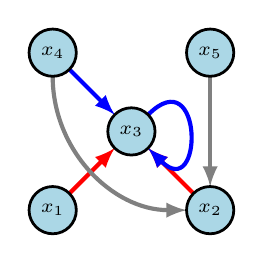
\begin{tikzpicture}
\Vertex[label=$x_{1}$]{A}
\Vertex[x=2,label=$x_{2}$]{B}
\Vertex[x=1,y=1,label=$x_{3}$]{C}
\Vertex[x=0,y=2,label=$x_{4}$]{D}
\Vertex[x=2,y=2,label=$x_{5}$]{E}
\Edge[Math,Direct=true,color=red](A)(C)
\Edge[Math,Direct=true,color=red](B)(C)
\Edge[Math,Direct=true,color=blue](C)(C)
\Edge[Math,Direct=true,color=blue](D)(C)
\Edge[Math,Direct=true,bend=-45,color=gray](D)(B)
\Edge[Math,Direct=true,color=gray](E)(B)
\end{tikzpicture}
\end{center}

Consider then, at $t=0$ we know the how many of each species are in $\Omega$: $\mathbf{X_{0}}$ and we would like to predict $\mathbf{X}_{t}$ at some $t > 0$. Since the evolution of the system is stochastic and the state space is discrete, we have to rely on master equations. Recall the general form of a master equation for a stochastic system where the state space is discrete

\begin{equation*}
J_{i} = \frac{dP_{i}}{dt} = \sum_{j} W_{ji}P_{j} - W_{ij}P_{i}
\end{equation*}

which, in words, reads that the probability current $J_{i}$ into the state $i$ is a sum over outgoing current $W_{ij}P_{i}$ into all other states $j$ and inward current $W_{ji}P_{j}$ from all other states $j$. The matrix $W$ is the so-called \emph{transition matrix}. In terms of chemical reactions, a transition between states $i$ and $j$ occurs via a single chemical reaction which occurs with a probability $a_{j}(\mathbf{x})$ dependent on the current state of the system

\begin{equation*}
\frac{dP(\mathbf{x},t)}{dt} = \sum_{j} a_{j}(\mathbf{x}-\nu_{j})P(\mathbf{x}-\nu_{j},t) - a_{j}(\mathbf{x})P(\mathbf{x},t)
\end{equation*}

The function $a_{j}(\mathbf{x})$ is generally defined as $a_{j}(\mathbf{x}) = c_{j}h_{j}(\mathbf{x})$ where $c_{j}$ is a constant factor specific to reaction $j$ while $h_{j}(\mathbf{x})$ is the number of distinct possible combinations of the reactants available in state $\mathbf{x}$. For example, for $r_{1}$ above, we have $h_{j}(\mathbf{x}) = x_{1}x_{2}$.

\subsubsection{The Gillespie algorithm}

The chemical master equation is notoriously difficult to solve, and in most cases, we need to simulate from $P(\mathbf{x},t)$ using Monte Carlo methods. Gillespie developed a method for simulating from $P(\mathbf{x},t)$, starting with the following questions: (1) when will the next chemical reaction occur and (2) what kind of reaction will it be? The algorithm proceeds by defining a joint density function $P(\tau,\mu)d\tau$ which describes the probability that the next reaction will be of type $\mu$ and occur and a time $\tau$. 

\subsubsection{Stability analysis of stochastic differential equations}

\subsubsection{Inferring biochemical networks from data}

\subsubsection{Learning interaction functions with Gaussian Processes}

\subsection{Experimental Methods}

\subsubsection{Multiplexed fluorescence in-situ hybridization (FISH)}

\subsubsection{Techniques for high-throughput image processing}

\bibliography{sample}

\end{document}